
% Default to the notebook output style

    


% Inherit from the specified cell style.




    
\documentclass[11pt]{article}

    
    
    \usepackage[T1]{fontenc}
    % Nicer default font (+ math font) than Computer Modern for most use cases
    \usepackage{mathpazo}

    % Basic figure setup, for now with no caption control since it's done
    % automatically by Pandoc (which extracts ![](path) syntax from Markdown).
    \usepackage{graphicx}
    % We will generate all images so they have a width \maxwidth. This means
    % that they will get their normal width if they fit onto the page, but
    % are scaled down if they would overflow the margins.
    \makeatletter
    \def\maxwidth{\ifdim\Gin@nat@width>\linewidth\linewidth
    \else\Gin@nat@width\fi}
    \makeatother
    \let\Oldincludegraphics\includegraphics
    % Set max figure width to be 80% of text width, for now hardcoded.
    \renewcommand{\includegraphics}[1]{\Oldincludegraphics[width=.8\maxwidth]{#1}}
    % Ensure that by default, figures have no caption (until we provide a
    % proper Figure object with a Caption API and a way to capture that
    % in the conversion process - todo).
    \usepackage{caption}
    \DeclareCaptionLabelFormat{nolabel}{}
    \captionsetup{labelformat=nolabel}

    \usepackage{adjustbox} % Used to constrain images to a maximum size 
    \usepackage{xcolor} % Allow colors to be defined
    \usepackage{enumerate} % Needed for markdown enumerations to work
    \usepackage{geometry} % Used to adjust the document margins
    \usepackage{amsmath} % Equations
    \usepackage{amssymb} % Equations
    \usepackage{textcomp} % defines textquotesingle
    % Hack from http://tex.stackexchange.com/a/47451/13684:
    \AtBeginDocument{%
        \def\PYZsq{\textquotesingle}% Upright quotes in Pygmentized code
    }
    \usepackage{upquote} % Upright quotes for verbatim code
    \usepackage{eurosym} % defines \euro
    \usepackage[mathletters]{ucs} % Extended unicode (utf-8) support
    \usepackage[utf8x]{inputenc} % Allow utf-8 characters in the tex document
    \usepackage{fancyvrb} % verbatim replacement that allows latex
    \usepackage{grffile} % extends the file name processing of package graphics 
                         % to support a larger range 
    % The hyperref package gives us a pdf with properly built
    % internal navigation ('pdf bookmarks' for the table of contents,
    % internal cross-reference links, web links for URLs, etc.)
    \usepackage{hyperref}
    \usepackage{longtable} % longtable support required by pandoc >1.10
    \usepackage{booktabs}  % table support for pandoc > 1.12.2
    \usepackage[inline]{enumitem} % IRkernel/repr support (it uses the enumerate* environment)
    \usepackage[normalem]{ulem} % ulem is needed to support strikethroughs (\sout)
                                % normalem makes italics be italics, not underlines
    

    
    
    % Colors for the hyperref package
    \definecolor{urlcolor}{rgb}{0,.145,.698}
    \definecolor{linkcolor}{rgb}{.71,0.21,0.01}
    \definecolor{citecolor}{rgb}{.12,.54,.11}

    % ANSI colors
    \definecolor{ansi-black}{HTML}{3E424D}
    \definecolor{ansi-black-intense}{HTML}{282C36}
    \definecolor{ansi-red}{HTML}{E75C58}
    \definecolor{ansi-red-intense}{HTML}{B22B31}
    \definecolor{ansi-green}{HTML}{00A250}
    \definecolor{ansi-green-intense}{HTML}{007427}
    \definecolor{ansi-yellow}{HTML}{DDB62B}
    \definecolor{ansi-yellow-intense}{HTML}{B27D12}
    \definecolor{ansi-blue}{HTML}{208FFB}
    \definecolor{ansi-blue-intense}{HTML}{0065CA}
    \definecolor{ansi-magenta}{HTML}{D160C4}
    \definecolor{ansi-magenta-intense}{HTML}{A03196}
    \definecolor{ansi-cyan}{HTML}{60C6C8}
    \definecolor{ansi-cyan-intense}{HTML}{258F8F}
    \definecolor{ansi-white}{HTML}{C5C1B4}
    \definecolor{ansi-white-intense}{HTML}{A1A6B2}

    % commands and environments needed by pandoc snippets
    % extracted from the output of `pandoc -s`
    \providecommand{\tightlist}{%
      \setlength{\itemsep}{0pt}\setlength{\parskip}{0pt}}
    \DefineVerbatimEnvironment{Highlighting}{Verbatim}{commandchars=\\\{\}}
    % Add ',fontsize=\small' for more characters per line
    \newenvironment{Shaded}{}{}
    \newcommand{\KeywordTok}[1]{\textcolor[rgb]{0.00,0.44,0.13}{\textbf{{#1}}}}
    \newcommand{\DataTypeTok}[1]{\textcolor[rgb]{0.56,0.13,0.00}{{#1}}}
    \newcommand{\DecValTok}[1]{\textcolor[rgb]{0.25,0.63,0.44}{{#1}}}
    \newcommand{\BaseNTok}[1]{\textcolor[rgb]{0.25,0.63,0.44}{{#1}}}
    \newcommand{\FloatTok}[1]{\textcolor[rgb]{0.25,0.63,0.44}{{#1}}}
    \newcommand{\CharTok}[1]{\textcolor[rgb]{0.25,0.44,0.63}{{#1}}}
    \newcommand{\StringTok}[1]{\textcolor[rgb]{0.25,0.44,0.63}{{#1}}}
    \newcommand{\CommentTok}[1]{\textcolor[rgb]{0.38,0.63,0.69}{\textit{{#1}}}}
    \newcommand{\OtherTok}[1]{\textcolor[rgb]{0.00,0.44,0.13}{{#1}}}
    \newcommand{\AlertTok}[1]{\textcolor[rgb]{1.00,0.00,0.00}{\textbf{{#1}}}}
    \newcommand{\FunctionTok}[1]{\textcolor[rgb]{0.02,0.16,0.49}{{#1}}}
    \newcommand{\RegionMarkerTok}[1]{{#1}}
    \newcommand{\ErrorTok}[1]{\textcolor[rgb]{1.00,0.00,0.00}{\textbf{{#1}}}}
    \newcommand{\NormalTok}[1]{{#1}}
    
    % Additional commands for more recent versions of Pandoc
    \newcommand{\ConstantTok}[1]{\textcolor[rgb]{0.53,0.00,0.00}{{#1}}}
    \newcommand{\SpecialCharTok}[1]{\textcolor[rgb]{0.25,0.44,0.63}{{#1}}}
    \newcommand{\VerbatimStringTok}[1]{\textcolor[rgb]{0.25,0.44,0.63}{{#1}}}
    \newcommand{\SpecialStringTok}[1]{\textcolor[rgb]{0.73,0.40,0.53}{{#1}}}
    \newcommand{\ImportTok}[1]{{#1}}
    \newcommand{\DocumentationTok}[1]{\textcolor[rgb]{0.73,0.13,0.13}{\textit{{#1}}}}
    \newcommand{\AnnotationTok}[1]{\textcolor[rgb]{0.38,0.63,0.69}{\textbf{\textit{{#1}}}}}
    \newcommand{\CommentVarTok}[1]{\textcolor[rgb]{0.38,0.63,0.69}{\textbf{\textit{{#1}}}}}
    \newcommand{\VariableTok}[1]{\textcolor[rgb]{0.10,0.09,0.49}{{#1}}}
    \newcommand{\ControlFlowTok}[1]{\textcolor[rgb]{0.00,0.44,0.13}{\textbf{{#1}}}}
    \newcommand{\OperatorTok}[1]{\textcolor[rgb]{0.40,0.40,0.40}{{#1}}}
    \newcommand{\BuiltInTok}[1]{{#1}}
    \newcommand{\ExtensionTok}[1]{{#1}}
    \newcommand{\PreprocessorTok}[1]{\textcolor[rgb]{0.74,0.48,0.00}{{#1}}}
    \newcommand{\AttributeTok}[1]{\textcolor[rgb]{0.49,0.56,0.16}{{#1}}}
    \newcommand{\InformationTok}[1]{\textcolor[rgb]{0.38,0.63,0.69}{\textbf{\textit{{#1}}}}}
    \newcommand{\WarningTok}[1]{\textcolor[rgb]{0.38,0.63,0.69}{\textbf{\textit{{#1}}}}}
    
    
    % Define a nice break command that doesn't care if a line doesn't already
    % exist.
    \def\br{\hspace*{\fill} \\* }
    % Math Jax compatability definitions
    \def\gt{>}
    \def\lt{<}
    % Document parameters
    \title{04.06??B\_5-112?charging\_process?Julia}
    
    
    

    % Pygments definitions
    
\makeatletter
\def\PY@reset{\let\PY@it=\relax \let\PY@bf=\relax%
    \let\PY@ul=\relax \let\PY@tc=\relax%
    \let\PY@bc=\relax \let\PY@ff=\relax}
\def\PY@tok#1{\csname PY@tok@#1\endcsname}
\def\PY@toks#1+{\ifx\relax#1\empty\else%
    \PY@tok{#1}\expandafter\PY@toks\fi}
\def\PY@do#1{\PY@bc{\PY@tc{\PY@ul{%
    \PY@it{\PY@bf{\PY@ff{#1}}}}}}}
\def\PY#1#2{\PY@reset\PY@toks#1+\relax+\PY@do{#2}}

\expandafter\def\csname PY@tok@w\endcsname{\def\PY@tc##1{\textcolor[rgb]{0.73,0.73,0.73}{##1}}}
\expandafter\def\csname PY@tok@c\endcsname{\let\PY@it=\textit\def\PY@tc##1{\textcolor[rgb]{0.25,0.50,0.50}{##1}}}
\expandafter\def\csname PY@tok@cp\endcsname{\def\PY@tc##1{\textcolor[rgb]{0.74,0.48,0.00}{##1}}}
\expandafter\def\csname PY@tok@k\endcsname{\let\PY@bf=\textbf\def\PY@tc##1{\textcolor[rgb]{0.00,0.50,0.00}{##1}}}
\expandafter\def\csname PY@tok@kp\endcsname{\def\PY@tc##1{\textcolor[rgb]{0.00,0.50,0.00}{##1}}}
\expandafter\def\csname PY@tok@kt\endcsname{\def\PY@tc##1{\textcolor[rgb]{0.69,0.00,0.25}{##1}}}
\expandafter\def\csname PY@tok@o\endcsname{\def\PY@tc##1{\textcolor[rgb]{0.40,0.40,0.40}{##1}}}
\expandafter\def\csname PY@tok@ow\endcsname{\let\PY@bf=\textbf\def\PY@tc##1{\textcolor[rgb]{0.67,0.13,1.00}{##1}}}
\expandafter\def\csname PY@tok@nb\endcsname{\def\PY@tc##1{\textcolor[rgb]{0.00,0.50,0.00}{##1}}}
\expandafter\def\csname PY@tok@nf\endcsname{\def\PY@tc##1{\textcolor[rgb]{0.00,0.00,1.00}{##1}}}
\expandafter\def\csname PY@tok@nc\endcsname{\let\PY@bf=\textbf\def\PY@tc##1{\textcolor[rgb]{0.00,0.00,1.00}{##1}}}
\expandafter\def\csname PY@tok@nn\endcsname{\let\PY@bf=\textbf\def\PY@tc##1{\textcolor[rgb]{0.00,0.00,1.00}{##1}}}
\expandafter\def\csname PY@tok@ne\endcsname{\let\PY@bf=\textbf\def\PY@tc##1{\textcolor[rgb]{0.82,0.25,0.23}{##1}}}
\expandafter\def\csname PY@tok@nv\endcsname{\def\PY@tc##1{\textcolor[rgb]{0.10,0.09,0.49}{##1}}}
\expandafter\def\csname PY@tok@no\endcsname{\def\PY@tc##1{\textcolor[rgb]{0.53,0.00,0.00}{##1}}}
\expandafter\def\csname PY@tok@nl\endcsname{\def\PY@tc##1{\textcolor[rgb]{0.63,0.63,0.00}{##1}}}
\expandafter\def\csname PY@tok@ni\endcsname{\let\PY@bf=\textbf\def\PY@tc##1{\textcolor[rgb]{0.60,0.60,0.60}{##1}}}
\expandafter\def\csname PY@tok@na\endcsname{\def\PY@tc##1{\textcolor[rgb]{0.49,0.56,0.16}{##1}}}
\expandafter\def\csname PY@tok@nt\endcsname{\let\PY@bf=\textbf\def\PY@tc##1{\textcolor[rgb]{0.00,0.50,0.00}{##1}}}
\expandafter\def\csname PY@tok@nd\endcsname{\def\PY@tc##1{\textcolor[rgb]{0.67,0.13,1.00}{##1}}}
\expandafter\def\csname PY@tok@s\endcsname{\def\PY@tc##1{\textcolor[rgb]{0.73,0.13,0.13}{##1}}}
\expandafter\def\csname PY@tok@sd\endcsname{\let\PY@it=\textit\def\PY@tc##1{\textcolor[rgb]{0.73,0.13,0.13}{##1}}}
\expandafter\def\csname PY@tok@si\endcsname{\let\PY@bf=\textbf\def\PY@tc##1{\textcolor[rgb]{0.73,0.40,0.53}{##1}}}
\expandafter\def\csname PY@tok@se\endcsname{\let\PY@bf=\textbf\def\PY@tc##1{\textcolor[rgb]{0.73,0.40,0.13}{##1}}}
\expandafter\def\csname PY@tok@sr\endcsname{\def\PY@tc##1{\textcolor[rgb]{0.73,0.40,0.53}{##1}}}
\expandafter\def\csname PY@tok@ss\endcsname{\def\PY@tc##1{\textcolor[rgb]{0.10,0.09,0.49}{##1}}}
\expandafter\def\csname PY@tok@sx\endcsname{\def\PY@tc##1{\textcolor[rgb]{0.00,0.50,0.00}{##1}}}
\expandafter\def\csname PY@tok@m\endcsname{\def\PY@tc##1{\textcolor[rgb]{0.40,0.40,0.40}{##1}}}
\expandafter\def\csname PY@tok@gh\endcsname{\let\PY@bf=\textbf\def\PY@tc##1{\textcolor[rgb]{0.00,0.00,0.50}{##1}}}
\expandafter\def\csname PY@tok@gu\endcsname{\let\PY@bf=\textbf\def\PY@tc##1{\textcolor[rgb]{0.50,0.00,0.50}{##1}}}
\expandafter\def\csname PY@tok@gd\endcsname{\def\PY@tc##1{\textcolor[rgb]{0.63,0.00,0.00}{##1}}}
\expandafter\def\csname PY@tok@gi\endcsname{\def\PY@tc##1{\textcolor[rgb]{0.00,0.63,0.00}{##1}}}
\expandafter\def\csname PY@tok@gr\endcsname{\def\PY@tc##1{\textcolor[rgb]{1.00,0.00,0.00}{##1}}}
\expandafter\def\csname PY@tok@ge\endcsname{\let\PY@it=\textit}
\expandafter\def\csname PY@tok@gs\endcsname{\let\PY@bf=\textbf}
\expandafter\def\csname PY@tok@gp\endcsname{\let\PY@bf=\textbf\def\PY@tc##1{\textcolor[rgb]{0.00,0.00,0.50}{##1}}}
\expandafter\def\csname PY@tok@go\endcsname{\def\PY@tc##1{\textcolor[rgb]{0.53,0.53,0.53}{##1}}}
\expandafter\def\csname PY@tok@gt\endcsname{\def\PY@tc##1{\textcolor[rgb]{0.00,0.27,0.87}{##1}}}
\expandafter\def\csname PY@tok@err\endcsname{\def\PY@bc##1{\setlength{\fboxsep}{0pt}\fcolorbox[rgb]{1.00,0.00,0.00}{1,1,1}{\strut ##1}}}
\expandafter\def\csname PY@tok@kc\endcsname{\let\PY@bf=\textbf\def\PY@tc##1{\textcolor[rgb]{0.00,0.50,0.00}{##1}}}
\expandafter\def\csname PY@tok@kd\endcsname{\let\PY@bf=\textbf\def\PY@tc##1{\textcolor[rgb]{0.00,0.50,0.00}{##1}}}
\expandafter\def\csname PY@tok@kn\endcsname{\let\PY@bf=\textbf\def\PY@tc##1{\textcolor[rgb]{0.00,0.50,0.00}{##1}}}
\expandafter\def\csname PY@tok@kr\endcsname{\let\PY@bf=\textbf\def\PY@tc##1{\textcolor[rgb]{0.00,0.50,0.00}{##1}}}
\expandafter\def\csname PY@tok@bp\endcsname{\def\PY@tc##1{\textcolor[rgb]{0.00,0.50,0.00}{##1}}}
\expandafter\def\csname PY@tok@fm\endcsname{\def\PY@tc##1{\textcolor[rgb]{0.00,0.00,1.00}{##1}}}
\expandafter\def\csname PY@tok@vc\endcsname{\def\PY@tc##1{\textcolor[rgb]{0.10,0.09,0.49}{##1}}}
\expandafter\def\csname PY@tok@vg\endcsname{\def\PY@tc##1{\textcolor[rgb]{0.10,0.09,0.49}{##1}}}
\expandafter\def\csname PY@tok@vi\endcsname{\def\PY@tc##1{\textcolor[rgb]{0.10,0.09,0.49}{##1}}}
\expandafter\def\csname PY@tok@vm\endcsname{\def\PY@tc##1{\textcolor[rgb]{0.10,0.09,0.49}{##1}}}
\expandafter\def\csname PY@tok@sa\endcsname{\def\PY@tc##1{\textcolor[rgb]{0.73,0.13,0.13}{##1}}}
\expandafter\def\csname PY@tok@sb\endcsname{\def\PY@tc##1{\textcolor[rgb]{0.73,0.13,0.13}{##1}}}
\expandafter\def\csname PY@tok@sc\endcsname{\def\PY@tc##1{\textcolor[rgb]{0.73,0.13,0.13}{##1}}}
\expandafter\def\csname PY@tok@dl\endcsname{\def\PY@tc##1{\textcolor[rgb]{0.73,0.13,0.13}{##1}}}
\expandafter\def\csname PY@tok@s2\endcsname{\def\PY@tc##1{\textcolor[rgb]{0.73,0.13,0.13}{##1}}}
\expandafter\def\csname PY@tok@sh\endcsname{\def\PY@tc##1{\textcolor[rgb]{0.73,0.13,0.13}{##1}}}
\expandafter\def\csname PY@tok@s1\endcsname{\def\PY@tc##1{\textcolor[rgb]{0.73,0.13,0.13}{##1}}}
\expandafter\def\csname PY@tok@mb\endcsname{\def\PY@tc##1{\textcolor[rgb]{0.40,0.40,0.40}{##1}}}
\expandafter\def\csname PY@tok@mf\endcsname{\def\PY@tc##1{\textcolor[rgb]{0.40,0.40,0.40}{##1}}}
\expandafter\def\csname PY@tok@mh\endcsname{\def\PY@tc##1{\textcolor[rgb]{0.40,0.40,0.40}{##1}}}
\expandafter\def\csname PY@tok@mi\endcsname{\def\PY@tc##1{\textcolor[rgb]{0.40,0.40,0.40}{##1}}}
\expandafter\def\csname PY@tok@il\endcsname{\def\PY@tc##1{\textcolor[rgb]{0.40,0.40,0.40}{##1}}}
\expandafter\def\csname PY@tok@mo\endcsname{\def\PY@tc##1{\textcolor[rgb]{0.40,0.40,0.40}{##1}}}
\expandafter\def\csname PY@tok@ch\endcsname{\let\PY@it=\textit\def\PY@tc##1{\textcolor[rgb]{0.25,0.50,0.50}{##1}}}
\expandafter\def\csname PY@tok@cm\endcsname{\let\PY@it=\textit\def\PY@tc##1{\textcolor[rgb]{0.25,0.50,0.50}{##1}}}
\expandafter\def\csname PY@tok@cpf\endcsname{\let\PY@it=\textit\def\PY@tc##1{\textcolor[rgb]{0.25,0.50,0.50}{##1}}}
\expandafter\def\csname PY@tok@c1\endcsname{\let\PY@it=\textit\def\PY@tc##1{\textcolor[rgb]{0.25,0.50,0.50}{##1}}}
\expandafter\def\csname PY@tok@cs\endcsname{\let\PY@it=\textit\def\PY@tc##1{\textcolor[rgb]{0.25,0.50,0.50}{##1}}}

\def\PYZbs{\char`\\}
\def\PYZus{\char`\_}
\def\PYZob{\char`\{}
\def\PYZcb{\char`\}}
\def\PYZca{\char`\^}
\def\PYZam{\char`\&}
\def\PYZlt{\char`\<}
\def\PYZgt{\char`\>}
\def\PYZsh{\char`\#}
\def\PYZpc{\char`\%}
\def\PYZdl{\char`\$}
\def\PYZhy{\char`\-}
\def\PYZsq{\char`\'}
\def\PYZdq{\char`\"}
\def\PYZti{\char`\~}
% for compatibility with earlier versions
\def\PYZat{@}
\def\PYZlb{[}
\def\PYZrb{]}
\makeatother


    % Exact colors from NB
    \definecolor{incolor}{rgb}{0.0, 0.0, 0.5}
    \definecolor{outcolor}{rgb}{0.545, 0.0, 0.0}



    
    % Prevent overflowing lines due to hard-to-break entities
    \sloppy 
    % Setup hyperref package
    \hypersetup{
      breaklinks=true,  % so long urls are correctly broken across lines
      colorlinks=true,
      urlcolor=urlcolor,
      linkcolor=linkcolor,
      citecolor=citecolor,
      }
    % Slightly bigger margins than the latex defaults
    
    \geometry{verbose,tmargin=1in,bmargin=1in,lmargin=1in,rmargin=1in}
    
    

    \begin{document}
    
    
    \maketitle
    
    

    
    \(\LaTeX\){ }

\(\require{cancel} \require{mhchem} \require{bbox} \require{color} \require{enclose} \require{AMSmath} \require{AMSsymbols}\)

    Çengel, Y. A., and Boles, M. A. (2001). Thermodynamics: An engineering
approach. Boston: McGraw-Hill.

    \textbf{5.112.} A 2 m³ rigid insulated tank initially containing
saturated water vapor at 1 MPa is connected through a valve to a supply
line that carries steam at 400 °C. Now the valve is opened, and steam is
allowed to flow slowly into the tank until the pressure in the tank
rises to 2 MPa. At this instant the tank temperature is measured to be
300 °C. Determine the mass of the steam that has entered and the
pressure of the steam in the supply line.

\begin{figure}
\centering
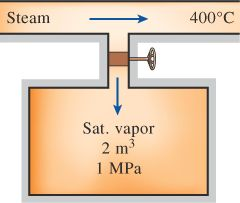
\includegraphics{./figures/ch05_cen98179_p05112_lg.7cc78c1912f24303ba7787713d5784c1.jpg}
\caption{Cengelboles7ed4-126}
\end{figure}

    \hypertarget{given}{%
\subsubsection{Given}\label{given}}

\begin{enumerate}
\def\labelenumi{\arabic{enumi}.}
\item
  \(V = 2\, m^3 \\[6pt]\)
\item
  \(T_{supply} = 400\, \text{°C} \\[6pt]\)
\item
  \(\ce{H2O} \left\{ \begin{align*}  P_{initial} &= 1\, \text{MPa} \\  x_{initial} &= 1 \end{align*} \right. \quad \Longrightarrow \quad\)
  \$ \left\{ \begin{align*} 
     P_{final} &= 2\, \text{MPa} \\
     T_{final}  &=  300\, \text{°C}
  \end{align*} \right. \$
\end{enumerate}

    \hypertarget{find}{%
\subsubsection{Find}\label{find}}

\begin{enumerate}
\def\labelenumi{\arabic{enumi}.}
\tightlist
\item
  \(m_{in}\)\\
\item
  \(P_{supply}\)
\end{enumerate}

    \hypertarget{get-organized}{%
\subsubsection{Get Organized}\label{get-organized}}

    First, we observe that this is NOT a steady state process. Energy and/or
mass of the system are changing in time. Remember, we must account for
our system spatially and temporally. It's not difficult if you stay
organized. We are given enough information to resolve two of the three
states we need (\emph{initial, final, supply}). Let's go through all the
information we need to find in order to answer the questions.\\

\begin{enumerate}
\def\labelenumi{\arabic{enumi}.}
\tightlist
\item
  \textbf{Mass entered, \(m_{in}\)}\\
  Apply continuity (aka conservation of mass)
\end{enumerate}

\textbackslash{}begin\{array\}\{ccccc\} m\_\{in\} \&-\& m\_\{out\} \&=\&
\Delta m\_\{sys\} \textbackslash{}{[}6pt{]} m\_\{in\} \&\& \&=\&
m\_\{final\} - m\_\{initial\} \textbackslash{}{[}6pt{]} m\_\{in\} \&\&
\&=\& \displaystyle \frac{V}{v_{final}} - \frac{V}{v_{initial}}
\textbackslash{} \textbackslash{}end\{array\}

We get \(m_{in}\) once we resolve initial and final states.

    \begin{enumerate}
\def\labelenumi{\arabic{enumi}.}
\setcounter{enumi}{1}
\tightlist
\item
  \textbf{Supply pressure \(P_{supply}\)}
\end{enumerate}

We can determine supply pressure by resolving the state of the supply
steam. For this, we apply the conservation of energy. We already know
\(T_{supply},\) so we can resolve the state with an independant
property. If the steam were modeled as an ideal gas, we would have other
options, but we try to avoid using the ideal gas approach with any
fluids that may change phase, like \textbf{STEAM}. \$
\textbackslash{}{[}12pt{]}\$

note

\$ ~\$ Typically, in unsteady flow systems, you cannot eliminate mass
terms via division. Stay vigilant.

\textbackslash{}begin\{array\}\{ccccc\} E\_\{in\} \&-\& E\_\{out\} \&=\&
\Delta E\_\{sys\} \textbackslash{}{[}6pt{]} H\_\{in\} \&\& \&=\&
U\_\{sys,final\} - U\_\{sys,initial\} \textbackslash{}{[}6pt{]}
m\_\{in\} h\_\{supply\} \&\& \&=\& m\_\{final\} u\_\{final\} -
m\_\{initial\} u\_\{initial\} \textbackslash{}{[}6pt{]}
\textbackslash{}end\{array\}

We calculated the mass terms already. We get \(u_{initial}\) and
\(u_{final}\) from the tables. Enthapy and pressure are independent, so
solve the energy equation for \(h_{supply},\) then use it to find
\(P_{supply}.\)

    \hypertarget{attack}{%
\section{Attack}\label{attack}}

    Today, we'll use Julia, with \emph{Unitful.jl}, a package for
calculation with physical units.

    \begin{Verbatim}[commandchars=\\\{\}]
{\color{incolor}In [{\color{incolor}1}]:} \PY{k}{using} \PY{n}{Unitful}\PY{p}{;}       \PY{c}{\PYZsh{} Unitful units package}
\end{Verbatim}


    Look up your properties, and get to work.

\(\quad \ce{H2O} \left| \begin{array}{ll}  \begin{subarray}{l}{\textit{1 MPa}}\\{\textit{sat vapor}}\end{subarray} & v_{initial} = 0.1944\, \ce{m^3/kg} & u_{initial} = 2583.6\, \ce{kJ/kg} \\  \begin{subarray}{l}{\textit{2 MPa}}\\{\textit{300 °C}}\end{subarray} & v_{final} = 0.1254\, \ce{m^3/kg} & u_{final} = 2772.15\, \ce{kJ/kg}  \end{array}\right.\)

    \begin{Verbatim}[commandchars=\\\{\}]
{\color{incolor}In [{\color{incolor}2}]:} \PY{n}{v\PYZus{}initial} \PY{o}{=} \PY{l+m+mf}{0.1944}\PY{n}{u}\PY{l+s}{\PYZdq{}}\PY{l+s}{m}\PY{l+s}{\PYZca{}}\PY{l+s}{3}\PY{l+s}{/}\PY{l+s}{k}\PY{l+s}{g}\PY{l+s}{\PYZdq{}}
        \PY{n}{v\PYZus{}final} \PY{o}{=} \PY{l+m+mf}{0.1254}\PY{n}{u}\PY{l+s}{\PYZdq{}}\PY{l+s}{m}\PY{l+s}{\PYZca{}}\PY{l+s}{3}\PY{l+s}{/}\PY{l+s}{k}\PY{l+s}{g}\PY{l+s}{\PYZdq{}}
        \PY{n}{u\PYZus{}initial} \PY{o}{=} \PY{l+m+mf}{2583.6}\PY{n}{u}\PY{l+s}{\PYZdq{}}\PY{l+s}{k}\PY{l+s}{J}\PY{l+s}{/}\PY{l+s}{k}\PY{l+s}{g}\PY{l+s}{\PYZdq{}}
        \PY{n}{u\PYZus{}final} \PY{o}{=} \PY{l+m+mf}{2772.15}\PY{n}{u}\PY{l+s}{\PYZdq{}}\PY{l+s}{k}\PY{l+s}{J}\PY{l+s}{/}\PY{l+s}{k}\PY{l+s}{g}\PY{l+s}{\PYZdq{}}\PY{p}{;}
\end{Verbatim}


    ~

    \begin{enumerate}
\def\labelenumi{\arabic{enumi}.}
\tightlist
\item
  \textbf{Mass entered, \(m_{in}\)}
\end{enumerate}

\(\displaystyle m_{in} = m_{final} - m_{initial} = \frac{V}{v_{final}} - \frac{V}{v_{initial}}\)

    \begin{Verbatim}[commandchars=\\\{\}]
{\color{incolor}In [{\color{incolor}3}]:} \PY{n}{V} \PY{o}{=} \PY{l+m+mi}{2}\PY{n}{u}\PY{l+s}{\PYZdq{}}\PY{l+s}{m}\PY{l+s}{\PYZca{}}\PY{l+s}{3}\PY{l+s}{\PYZdq{}}  \PY{c}{\PYZsh{} Given}
        
        \PY{n}{m\PYZus{}initial} \PY{o}{=} \PY{n}{V} \PY{o}{/} \PY{n}{v\PYZus{}initial}
        \PY{n}{m\PYZus{}final} \PY{o}{=} \PY{n}{V} \PY{o}{/} \PY{n}{v\PYZus{}final}
        
        \PY{n}{m\PYZus{}in} \PY{o}{=} \PY{n}{m\PYZus{}final} \PY{o}{\PYZhy{}} \PY{n}{m\PYZus{}initial}
\end{Verbatim}


\begin{Verbatim}[commandchars=\\\{\}]
{\color{outcolor}Out[{\color{outcolor}3}]:} 5.660897473762969 kg
\end{Verbatim}
            
    1

\(\ \normalsize m_{in} = 5.661\, \ce{kg}\)

    ~

    \begin{enumerate}
\def\labelenumi{\arabic{enumi}.}
\setcounter{enumi}{1}
\tightlist
\item
  \textbf{Supply pressure \(P_{supply}\)}
\end{enumerate}

Solve the energy equation for \(h_{supply},\) then use it to find
\(P_{supply}.\)

\$ \displaystyle h\_\{supply\} =
\frac{m_{final} u_{final} - m_{initial} u_{initial}}{m_{in}} \$

    \begin{Verbatim}[commandchars=\\\{\}]
{\color{incolor}In [{\color{incolor}4}]:} \PY{n}{h\PYZus{}supply} \PY{o}{=} \PY{p}{(}\PY{n}{m\PYZus{}final}\PY{o}{*}\PY{n}{u\PYZus{}final} \PY{o}{\PYZhy{}} \PY{n}{m\PYZus{}initial}\PY{o}{*}\PY{n}{u\PYZus{}initial}\PY{p}{)} \PY{o}{/} \PY{n}{m\PYZus{}in}
\end{Verbatim}


\begin{Verbatim}[commandchars=\\\{\}]
{\color{outcolor}Out[{\color{outcolor}4}]:} 3114.8191304347824 kJ kg\^{}-1
\end{Verbatim}
            
    Now, set the final state for the steam supply.
\(\quad \ce{H2O}\left|\small \begin{array}{ll} T = 400\, °C  \\[-12pt] h = 3114.819\, \ce{kJ/kg} \end{array} \right.\)

We have to interpolate in the superheat table to determine the pressure.
Find two states at 400 °C with enthalpies that bracket \(h_{supply}.\)

\$\ce{H2O}\left\textbar{}\_\{400, °C\}\right. \quad \small 

\begin{array}{c|c|c|l} 
      P & 80\, & 100 & \ce{bar} \\[-12pt] 
      h & 3138.3\,  &3096.5 & \ce{kJ/kg} \end{array}

\$

    \begin{Verbatim}[commandchars=\\\{\}]
{\color{incolor}In [{\color{incolor}5}]:} \PY{n}{P} \PY{o}{=} \PY{p}{[}  \PY{l+m+mi}{80}     \PY{l+m+mi}{100}  \PY{p}{]}\PY{n}{u}\PY{l+s}{\PYZdq{}}\PY{l+s}{b}\PY{l+s}{a}\PY{l+s}{r}\PY{l+s}{\PYZdq{}}
        \PY{n}{h} \PY{o}{=} \PY{p}{[}\PY{l+m+mf}{3138.3}  \PY{l+m+mf}{3096.5}\PY{p}{]}\PY{n}{u}\PY{l+s}{\PYZdq{}}\PY{l+s}{k}\PY{l+s}{J}\PY{l+s}{/}\PY{l+s}{k}\PY{l+s}{g}\PY{l+s}{\PYZdq{}}
        
        \PY{n}{P\PYZus{}supply} \PY{o}{=} \PY{n}{P}\PY{p}{[}\PY{l+m+mi}{1}\PY{p}{]} \PY{o}{+} \PY{p}{(}\PY{n}{P}\PY{p}{[}\PY{l+m+mi}{2}\PY{p}{]} \PY{o}{\PYZhy{}} \PY{n}{P}\PY{p}{[}\PY{l+m+mi}{1}\PY{p}{]}\PY{p}{)}\PY{o}{*}\PY{p}{(}\PY{n}{h\PYZus{}supply} \PY{o}{\PYZhy{}} \PY{n}{h}\PY{p}{[}\PY{l+m+mi}{1}\PY{p}{]}\PY{p}{)} \PY{o}{/} \PY{p}{(}\PY{n}{h}\PY{p}{[}\PY{l+m+mi}{2}\PY{p}{]} \PY{o}{\PYZhy{}} \PY{n}{h}\PY{p}{[}\PY{l+m+mi}{1}\PY{p}{]}\PY{p}{)}
\end{Verbatim}


\begin{Verbatim}[commandchars=\\\{\}]
{\color{outcolor}Out[{\color{outcolor}5}]:} 91.2348658206783 bar
\end{Verbatim}
            
    2

\(\ \normalsize P_{supply} = 91.23\, \ce{bar}\)

    ψᵟ


    % Add a bibliography block to the postdoc
    
    
    
    \end{document}
